%!TEX root = ../thesis.tex

\chapter{Top Quark mass measurement}
\label{c:top_mass_analysis}
\ifpdf
    \graphicspath{{05_Mass_analysis/plots/}}
\else
    \graphicspath{{05_Mass_analysis/plots/EPS/}{05_Mass_analysis/plots/}}
\fi

In this chapter the top mass measurement using 2011 LHC data recorded by the CMS detector at a centre of mass energy of
$\sqrt s =$ \SI{7}{\TeV} is presented. This analysis was a cross-check of the official CMS top mass measurement at
\SI{7}{\TeV} in lepton plus jets channel published in 2012 \autocite{top_mass_ljets_CMS}. Only the electron channel is
described here, as the muon side of this analysis was performed by a different group at CERN, although in close
collaboration.

The mass extraction method used in this analysis is essentially the same to one used in the CMS measurement of the mass
difference between top and antitop quarks \autocite{mass_difference_CMS} and top mass measurement in 2010
\autocite{top_mass_ljets_CMS_2010}.

%talk about JES limiting factor, why the analysis is a cross check, why is it important, cite the main CMS paper, a
%couple of words about the ideogram method... anything else? theory motivation should be in the first chapter,
%reference it.

\section{Data and Simulation}
\label{s_top_mass:data_and_simulation}

\subsection{Data}
\label{ss_top_mass:data}
This analysis uses the full 2011 data recorded by the CMS detector with a total integrated luminosity of
\SI{5.0 \pm 0.1}{\fbinv}. As only the electron channel is covered by this particular analysis, all data was pre-selected
by single electron plus jets high level triggers, described in detail in Chapter \ref{c:service_work}.

% \begin{itemize}
%   \item electron + 3 (PF)jets
%   \item isolated electron + 3 (PF)jets
% \end{itemize}

% \begin{itemize}
% 	\item /ElectronHad/Run2011A-May10ReReco-v1/AOD
% 	\item /ElectronHad/Run2011A-PromptReco-v4/AOD
% 	\item /ElectronHad/Run2011A-05Aug2011-v1/AOD
% 	\item /ElectronHad/Run2011A-PromptReco-v6/AOD
% 	\item /ElectronHad/Run2011B-PromptReco-v1/AOD
% \end{itemize}

\subsection{Simulation of signal and background processes}
\label{ss_top_mass:signal_and_background}

To develop and test any analysis technique, simulated events from Monte Carlo (MC) generators are inevitably needed. In
this work the \ttbar signal and W+Jets background events were generated with the MadGraph matrix element generator
\autocite{MadGraph}, Pythia parton showering \autocite{Pythia} and a full GEANT4-based detector simulation
\autocite{GEANT4}. The single top background was simulated using Powheg \autocite{POWHEG}. Let us briefly describe these
generators.

% The \ttbar signal is available with 9 different generated top quark masses and
% systematic variations. Pile up reweighting is used to match the simulation to the vertex multiplicity in data. The
% MC/data differences of b-tagging efficiencies and trigger efficiencies are taken into account by additional MC scale
% factors. The jet energy resolution is scaled to match the resolution in data.

% Signal:
% \begin{itemize}
% \item {\footnotesize /TTJets\_TuneZ2\_mass161\_5\_7TeV-madgraph-tauola/Fall11-PU\_S6\_START42\_V14B-v3/AODSIM}
% \item {\footnotesize /TTJets\_TuneZ2\_mass163\_5\_7TeV-madgraph-tauola/Summer11-PU\_S4\_START42\_V11-v3/AODSIM}
% \item {\footnotesize /TTJets\_TuneZ2\_mass166\_5\_7TeV-madgraph-tauola/Summer11-PU\_S4\_START42\_V11-v3/AODSIM}
% \item {\footnotesize /TTJets\_TuneZ2\_mass169\_5\_7TeV-madgraph-tauola/Summer11-PU\_S4\_START42\_V11-v3/AODSIM}
% \item {\footnotesize /TTJets\_TuneZ2\_7TeV-madgraph-tauola/Fall11-PU\_S6\_START42\_V14B-v2/AODSIM}
% \item {\footnotesize /TTJets\_TuneZ2\_mass175\_5\_7TeV-madgraph-tauola/Summer11-PU\_S4\_START42\_V11-v3/AODSIM}
% \item {\footnotesize /TTJets\_TuneZ2\_mass178\_5\_7TeV-madgraph-tauola/Summer11-PU\_S4\_START42\_V11-v3/AODSIM}
% \item {\footnotesize /TTJets\_TuneZ2\_mass181\_5\_7TeV-madgraph-tauola/Summer11-PU\_S4\_START42\_V11-v3/AODSIM}
% \item {\footnotesize /TTJets\_TuneZ2\_mass184\_5\_7TeV-madgraph-tauola/Fall11-PU\_S6\_START42\_V14B-v1/AODSIM}
% \end{itemize}
% Background:
% \begin{itemize}
% \item {\footnotesize /QCD\_Pt-20\_MuEnrichedPt-15\_TuneZ2\_7TeV-pythia6/Fall11-PU\_S6\_START42\_V14B-v1/AODSIM}
% \item {\footnotesize /QCD\_Pt-20to30\_EMEnriched\_TuneZ2\_7TeV-pythia6/Fall11-PU\_S6\_START42\_V14B-v1/AODSIM}
% \item {\footnotesize /QCD\_Pt-30to80\_EMEnriched\_TuneZ2\_7TeV-pythia/Fall11-PU\_S6\_START42\_V14B-v1/AODSIM}
% \item {\footnotesize /QCD\_Pt-80to170\_EMEnriched\_TuneZ2\_7TeV-pythia6/Fall11-PU\_S6\_START42\_V14B-v2/AODSIM}
% \item {\footnotesize /QCD\_Pt-20to30\_BCtoE\_TuneZ2\_7TeV-pythia6/Fall11-PU\_S6\_START42\_V14B-v1/AODSIM}
% \item {\footnotesize /QCD\_Pt-30to80\_BCtoE\_TuneZ2\_7TeV-pythia6/Fall11-PU\_S6\_START42\_V14B-v1/AODSIM}
% \item {\footnotesize /QCD\_Pt-80to170\_BCtoE\_TuneZ2\_7TeV-pythia/Fall11-PU\_S6\_START42\_V14B-v1/AODSIM}
% \item {\footnotesize /WJetsToLNu\_TuneZ2\_7TeV-madgraph-tauola/Fall11-PU\_S6\_START42\_V14B-v1/AODSIM}
% \item {\footnotesize /DYJetsToLL\_TuneZ2\_M-50\_7TeV-madgraph-tauola/Fall11-PU\_S6\_START42\_V14B-v1/AODSIM}
% \item {\footnotesize /Tbar\_TuneZ2\_s-channel\_7TeV-powheg-tauola/Summer11-PU\_S4\_START42\_V11-v1/AODSIM}
% \item {\footnotesize /Tbar\_TuneZ2\_t-channel\_7TeV-powheg-tauola/Summer11-PU\_S4\_START42\_V11-v1/AODSIM}
% \item {\footnotesize /Tbar\_TuneZ2\_tW-channel-DR\_7TeV-powheg-tauola/Summer11-PU\_S4\_START42\_V11-v1/AODSIM}
% \item {\footnotesize /T\_TuneZ2\_s-channel\_7TeV-powheg-tauola/Summer11-PU\_S4\_START42\_V11-v1/AODSIM}
% \item {\footnotesize /T\_TuneZ2\_t-channel\_7TeV-powheg-tauola/Summer11-PU\_S4\_START42\_V11-v1/AODSIM}
% \item {\footnotesize /T\_TuneZ2\_tW-channel-DR\_7TeV-powheg-tauola/Summer11-PU\_S4\_START42\_V11-v1/AODSIM}
% \end{itemize}
% Systematic variations:
% \begin{itemize}
% \item {\footnotesize (/TTjets\_TuneZ2\_matchingdown\_7TeV-madgraph-tauola/Fall11-PU\_S4\_START42\_V11-v1/AODSIM)}
% \item {\footnotesize /TTjets\_TuneZ2\_matchingup\_7TeV-madgraph-tauola/Fall11-PU\_S6\_START42\_V14B-v2/AODSIM}
% \item {\footnotesize /TTjets\_TuneZ2\_scaledown\_7TeV-madgraph-tauola/Fall11-PU\_S6\_START42\_V14B-v2/AODSIM}
% \item {\footnotesize /TTjets\_TuneZ2\_scaleup\_7TeV-madgraph-tauola/Fall11-PU\_S6\_START42\_V14B-v1/AODSIM}
% \item {\footnotesize /TTJets\_TuneP11\_7TeV-madgraph-tauola/Fall11-PU\_S6\_START42\_V14B-v1/AODSIM}
% \item {\footnotesize (/TTJets\_TuneP11noCR\_7TeV-madgraph-tauola/Fall11-PU\_S6\_START42\_V14B-v1/AODSIM)}
% \end{itemize}

\subsection{Monte Carlo generators}
\label{ss_top_mass:MC_generators}

In order to simulate the previously described signal and background processes several Monte Carlo (MC) event generators
are used. Given the process the event generators produce the long chain needed for a event: production of the main
process; particle decays; boson radiation (\Z, \photon, \cPg); and the hadronisation of quarks and gluons. Each
generator is optimised in one or more aspects of this chain and is therefore either used in conjunction with another
generator (signal generation with \MADGRAPH + \PYTHIA) or used for modelling the systematic uncertainty on the theory
due to different prescriptions (\POWHEG + \PYTHIA, \MCATNLO). As a specialist in radiation and hadronisation \PYTHIA is
either used by itself (QCD \multijet events) or takes over from the other generators at this step.

\subsubsection*{MadGraph}

\MADGRAPH \autocite{MadGraph} is a matrix-element Monte Carlo event generator. For any renormalisable Lagrangian based
model it produces all possible Feynman diagrams and automatically generates its matrix elements at the tree-level,
performing the integration over all phase-space. This calculation is then used to produce the \xsect of various
processes and subprocesses as well as partons and kinematics of an event, including decays that are described using spin
correlations. The partons from matrix element calculations are then matched to parton showers from hadronisation of
quarks and gluons, which is simulated in \PYTHIA (see below) along with the fragmentation of initial protons and the
soft scattering of underlying event (see Section~\ref{sss:JEC}). The matching is done according to so-called MLM
prescription \autocite{MLM} if a parton-jet pair satisfies a certain $\Delta R$ separation criteria. If no or more than
one matched jets are found, events are rejected. There is also a certain transverse energy threshold requirement for the
partons to be considered in the matching. Default values depend on the process and are set to be \SI{20}{\GeV} for
\ttbar events and \SI{10}{\GeV} for \WpJets and \ZpJets events.

%An additional package (\TAUOLA \autocite{TAUOLA}) is used for tau lepton decay description.

\subsubsection*{PYTHIA} 

\PYTHIA \autocite{Pythia,Pythia6.4} is perhaps the most widely used MC generator in high energy physics. It is a
standard tool used for simulation of quark and gluon hadronisation, multi-particle production, beam remnants, initial
protons fragmentation, etc. Therefore \PYTHIA is used to generate QCD multi-jet production and underlying event on top
of other generators providing partons from hard processes.

\subsubsection*{POWHEG} 

\POWHEG (Positive Weight Hardest Emission Generator) \autocite{POWHEG} was proposed to overcome the problem of negative
event weights which arise in the \MCATNLO method when matching NLO QCD computations with parton showers. Compared to
other generators \POWHEG generates the hardest radiation first. This is done with a technique that yields only
positive-weighted events using the exact NLO matrix elements.

\subsection{Factorisation Scale and Matching Threshold}
\label{ss:factorisation_and_matching}
%https://twiki.cern.ch/twiki/bin/view/CMS/MadGraphStandardModel

As previously described, the matching between the partons from the matrix-element calculations and the parton showers is
performed only for partons which exceed a transverse energy threshold. The systematic uncertainty resulting from the
choice of this threshold is estimated by using samples that have been produced with half and double the chosen
threshold. A similar procedure is deployed for the choice of the factorisation scale, which determines the scale at
which $\alpS$ is evaluated.
A summary of the used values for the uncertainty calculation is shown in table.


\subsection{Detector simulation with GEANT}
After the full physics simulation the last important step of the simulation process is the simulation of the detector
and its interaction with the generated particles. This process is performed in the detector simulation package
\GEANTfour (GEometry ANd Tracking) \autocite{GEANT4}. \GEANTfour recreates the geometry of the detector, describes the
material in the detector and particle interactions within it such as tracking and detector response.

\subsection{Monte Carlo samples}
The simulated MC events are generated at the center of mass energy of \SI{7}{\TeV}, using the CTEQ6L Parton Distribution
Functions (PDF) \autocite{CTEQ}. They are produced separately for each process. The \zp signal as well as the main
background processes are simulated in \MADGRAPH. Signal samples are produced with various masses and widths of the \zp
boson (see table \ref{tab:top_mass_signal_mc}). To extend the available statistics for the \WpJets sample four
additional \WpJets samples are included. These samples are generated in exclusive jet multiplicity bins: \W boson
production plus with one/two/three and at least four jets.

The QCD background samples are generated in \PYTHIA while the \photon + jets samples are generated with \MADGRAPH (table
\ref{tab:top_mass_background_qcd}). Since only a small fraction of the QCD \multijet events is of use in this analysis,
samples with generator level cuts are used to enhance the available statistics after the selection. These samples either
contain jets with high electromagnetic content (EM-enriched) or contain heavy flavour quarks (b or c) which decay into
electron plus neutrino ($\cPqb/\cPqc \rightarrow \cPq e\nu$). These two sets of QCD samples are generated in different
bins of $\hat\pt$ where most events surviving the selection come from the high bins. $\hat\pt$ denotes the transverse
momentum of the partons produced. The \photon plus jets samples are generated in different bins of \HT, defined as the
sum of transverse momenta of all particles.

\begin{table}[!htbp]
\centering
\caption{Signal and background Monte Carlo samples with cross sections at $\sqrt s = \SI{7}{\TeV}$, numbers of generated
events and corresponding integrated luminosities.}
\label{tab:top_mass_mc_samples}
\begin{tabular}{|l|l|r|r|r|}
\toprule
Process & Generator & $\sigma$ (\pb) & \# events & $\int\lumi dt$ (\fbinv)\\
\midrule
\ttjets & \MADGRAPH & & & \\
\hspace{5 mm}\mtop = \SI{161.5}{\GeV} & & 157.5 & 1620072 & 10.3\\
\hspace{5 mm}\mtop = \SI{163.5}{\GeV} & & 157.5 & 1633197 & 10.4\\
\hspace{5 mm}\mtop = \SI{166.5}{\GeV} & & 157.5 & 1669034 & 10.6\\
\hspace{5 mm}\mtop = \SI{169.5}{\GeV} & & 157.5 & 1606570 & 10.2\\
\hspace{5 mm}\mtop = \SI{172.5}{\GeV} & & 157.5 & 7490162 & 47.6\\
\hspace{5 mm}\mtop = \SI{175.5}{\GeV} & & 157.5 & 1538301 & 9.8\\
\hspace{5 mm}\mtop = \SI{178.5}{\GeV} & & 157.5 & 1648519 & 10.5\\
\hspace{5 mm}\mtop = \SI{181.5}{\GeV} & & 157.5 & 1665350 & 10.6\\
\hspace{5 mm}\mtop = \SI{184.5}{\GeV} & & 157.5 & 1671859 & 10.6\\
\midrule
\WpJets ($\W \rightarrow l\nu$) & \MADGRAPH & 31314 & 81345381 & 2.6 \\
% \hspace{5 mm}\W + 1 jet & & 4480 & 76051609 & 17.0 \\
% \hspace{5 mm}\W + 2 jet & & 1674 & 25400546 & 15.2 \\
% \hspace{5 mm}\W + 3 jet & & 484.7 & 7541595 & 15.6 \\
% \hspace{5 mm}\W + 4 jet & & 211.7 & 13133738 & 62.0 \\
\midrule
$\Z/\gamma^* \rightarrow l^+l^- $ + jets, $m(ll) > \SI{50}{\GeV}$ & \MADGRAPH & 3048 & 36222153 & 11.9 \\
\midrule
Single top & \POWHEG & & & \\
\hspace{5 mm} top $t$-channel & & 42.6 & 3814228 & 89.5 \\
\hspace{5 mm} anti-top $t$-channel & & 22.0 & 1944822 & 88.4 \\
\hspace{5 mm} top $s$-channel & & 2.72 & 259971 & 92.6 \\
\hspace{5 mm} anti-top $s$-channel & & 1.49 & 137980 & 92.6 \\
\hspace{5 mm} top $tW$-channel & & 5.3 & 814390 & 153.7 \\
\hspace{5 mm} anti-top $tW$-channel & & 5.3 & 809984 & 152.8 \\
\bottomrule
\end{tabular}
\end{table}

% \begin{table}[!hbth] \centering
% \begin{tabular}{lrrr}
% \toprule
% process & $\sigma$ (\pb) & \# events & $\int\lumi dt$ \fbinv\\
% \midrule
% \WpJets ($\W \rightarrow l\nu$) & 31314 & 81345381 & 2.6 \\
% \W + 1 jet ($\W \rightarrow l\nu$) & 4480 & 76051609 & 17.0 \\
% \W + 2 jet ($\W \rightarrow l\nu$) & 1674 & 25400546& 15.2 \\
% \W + 3 jet ($\W \rightarrow l\nu$) & 484.7 & 7541595 & 15.6 \\
% \W + 4 jet ($\W \rightarrow l\nu$) & 211.7 & 13133738 & 62.0 \\
% $\Z/\gamma^* \rightarrow l^+l^-, m(ll) > \SI{50}{\GeV}$ + jets & 3048 & 36222153 & 11.9 \\
% Single top t-channel & 42.6 & 3814228 & 89.5 \\
% Single anti-top t-channel & 22.0 & 1944822 & 88.4 \\
% Single top s-channel & 2.72 & 259971 & 92.6 \\
% Single anti-top s-channel & 1.49 & 137980 & 92.6 \\
% Single top tW-channel & 5.3 & 814390 & 153.7 \\
% Single anti-top tW-channel & 5.3 & 809984 & 152.8 \\
% \bottomrule
% \end{tabular}
% \caption{Background Monte Carlo samples, their cross sections at a \CoM energy
% of \SI{7}{\TeV}, numbers of generated events and corresponding integrated
% luminosities.}
% \label{tab:top_mass_background_mc}
% \end{table}

\begin{table}[!htbp] 
\centering
\caption{QCD multi-jet background and $\gamma$ + jets MC samples with cross sections at $\sqrt s =
\SI{7}{\TeV}$, numbers of generated events and corresponding integrated luminosities.
% EM-enriched samples are preselected to include jets with higher electromagnetic content;
% $\cPqb/\cPqc \rightarrow e\nu$ samples are preselected to include leptonic ($e\nu$) in-flight decays of b- and c-quarks.
}
\label{tab:top_mass_background_qcd}
\resizebox{\textwidth}{!}{
\begin{tabular}{|l|l|r|r|r|r|}
\toprule
Process & Generator & $\sigma$ (\pb) & filter efficiency & \# events & $\int\lumi dt$ (\fbinv)\\
\midrule
QCD ($e/\gamma$ enriched)  & \PYTHIA & & & & \\
\hspace{5 mm}\SIrange[range-phrase = $~<\pthat<~$]{20}{30}{\GeV} & & \num{2.355d8} & \num{7.3d-3} & 34720808 & \num{2.0d-2} \\
\hspace{5 mm}\SIrange[range-phrase = $~<\pthat<~$]{30}{80}{\GeV}  & & \num{5.93d7}& \num{0.059} &  70375915 & \num{2.0d-2} \\
\hspace{5 mm}\SIrange[range-phrase = $~<\pthat<~$]{80}{170}{\GeV} & & \num{9.06d5} & \num{0.148} &  8150669& \num{6.1d-2} \\
\midrule
QCD ($\cPqb/\cPqc \rightarrow e\nu$) & \PYTHIA & & & & \\
\hspace{5 mm}\SIrange[range-phrase = $~<\pthat<~$]{20}{30}{\GeV} & & \num{2.355d8} & \num{4.6d-4} & 2002588 & \num{1.8d-2} \\
\hspace{5 mm}\SIrange[range-phrase = $~<\pthat<~$]{30}{80}{\GeV} & & \num{5.93d7}& \num{2.34d-3} & 2030030 & \num{1.5d-2} \\
\hspace{5 mm}\SIrange[range-phrase = $~<\pthat<~$]{80}{170}{\GeV} & & \num{9.06d5} & \num{0.0104} & 1082690 & \num{0.1} \\
\midrule
$\gamma$ + jets & \MADGRAPH & & & & \\
\hspace{5 mm}\SIrange[range-phrase = $~<\HT<~$]{40}{100}{\GeV} & & \num{23620} & 1 & 12730863 & \num{0.5} \\
\hspace{5 mm}\SIrange[range-phrase = $~<\HT<~$]{100}{200}{\GeV} & & \num{3476} & 1 & 1536287 & \num{0.4} \\
\hspace{5 mm}$\HT >$ \SI{200}{\GeV} & & \num{485} & 1 & 9377168 & \num{19.3} \\
\bottomrule
\end{tabular}
}
\end{table}

\begin{table}[!htbp]
\centering
\caption{Systematic MC samples with cross sections at $\sqrt s = \SI{7}{\TeV}$, numbers of generated events and
corresponding integrated luminosities. Factorisation scale $Q$ and matching threshold systematic uncertainties (see
Section \ref{ss:matching_and_factorisation}) are estimated with variations of \ttjets, \WpJets and \ZpJets samples.}
\label{tab:top_mass_systematic_samples}
\begin{tabular}{|l|l|r|r|r|}
\toprule
Process & Generator & $\sigma$ (\pb) & \# events & $\int\lumi dt$ (\fbinv)\\
\midrule
\ttjets & \MADGRAPH & & & \\
\hspace{5 mm}$0.5~\times$ matching threshold & & 157.5 & 1607808& 10.2 \\
\hspace{5 mm}$2~\times$ matching threshold  & & 157.5 & 4029823& 25.5 \\
\hspace{5 mm}$0.5\times Q$  & & 157.5 & 4004587 & 25.4 \\
\hspace{5 mm}$2\times Q$ & & 157.5 & 3696269 & 23.4 \\
\midrule
\WpJets ($\W \rightarrow l\nu$) & \MADGRAPH & & & \\
\hspace{5 mm}$0.5~\times$ matching threshold & & 29690 & 9956679 & 0.3 \\
\hspace{5 mm}$2~\times$ matching threshold & & 30290 & 10461655 & 0.3 \\
\hspace{5 mm}$0.5 \times Q$ & & 33300 &10092532 & 0.3 \\
\hspace{5 mm}$2 \times Q$ & & 32000 &9784907 &0.3 \\
\midrule
\ZpJets ($\Z \rightarrow ll$) & \MADGRAPH & & & \\
\hspace{5 mm}$0.5~\times$ matching threshold & & 2888 & 1614808& 0.6 \\
\hspace{5 mm}$2~\times$ matching threshold & & 2915 & 1641121 & 0.6 \\
\hspace{5 mm}$0.5 \times Q$ & & 3312 & 1658855 & 0.5 \\
\hspace{5 mm}$2 \times Q$ & & 2954 & 1592742 & 0.5 \\
\bottomrule
\end{tabular}
\end{table}

\clearpage

\subsection{Pile-up reweighting}
\label{ss_top_mass:pileup_reweithing}

\subsection{b-tagging corrections}
\label{ss_top_mass:btagging_corrections}

\section{Event Selection}
\label{s_top_mass:event_selection}
Event selection applied in this analysis essentially follows the top quark group reference selection that is recommended
as a standard CMS top analyses selection optimised for SM \ttbar production. It is designed to select the semi-leptonic
signature of a \ttbar decay with an isolated lepton, four jets (including two jets from \cPqb-quarks) and a neutrino in
the form of missing transverse energy. All objects are reconstructed using the particle flow method as described in
Section~\ref{s:object_reconstruction}.

% and use the pile-up subtraction techniques for charged particles (no neutral particle correction) as described in
% Section %\ref{ss:pileup_subtraction}.

As this analysis focuses on the electron channel, the event selection proceeds as follows:

\begin{enumerate}[topsep=\parskip, parsep=\parskip, itemsep=\parskip, leftmargin=\leftmargin]
	\item preselection;
	\item trigger;
	\item electron candidate selection;
	\item dilepton veto;
	\item conversion veto;
	\item muon veto;
	\item jet selection;
	\item b-tagging.
\end{enumerate}

\subsubsection*{Preselection}
Preselection is performed in order to reduce the number of events stored for local analysis. All events are required to
have at least one electron with a \pt above \SI{30}{\GeV} or at least one muon with a \pt above \SI{20}{\GeV}.
Additional event cleaning is performed at this stage to decrease the number of events with substantial detector noise. A
small fraction of events with anomalous HCAL noise is removed by HCAL noise filter. Furthermore, beam scraping is
mitigated by the appropriate filter requiring at least \SI{25}{\percent} tracks with high purity if there are more than
\num{10} tracks in the event. Finally, preselection stage includes the requirement of at least one good primary vertex
in the event which has to be located within \SI{24}{\cm} in $z$-direction from the centre of CMS and within a radial
distance of \SI{2}{\cm}. The primary vertex is also required to have at least four degrees of freedom which is
determined from the vertex fit and is strongly correlated with the number of tracks compatible with the primary
interaction region \autocite{Tacking_PV_results_7TeV}.
%https://twiki.cern.ch/twiki/bin/view/CMS/TWikiTop2011DataMCTrig

\subsubsection*{Trigger}
The trigger requirement is imposed in a way it has been described in Chapter~\ref{c:service_work}. Essentially, all the
events are required to fire the electron-plus-three-jets trigger in its available version. A full list of triggers can
be found in the appendix \ref{s:full_trigger_list_electron}.

\subsubsection*{Electron candidate selection}
Exactly one electron candidate satisfying all following criteria is required to be present in the event. As soon as the
electron-plus-jets trigger has the lepton \pt threshold of \SI{25}{\GeV}, the electron candidate transverse momentum is
required to be above \SI{30}{\GeV} (in order to be in the trigger efficiency plateau region). Furthermore, the electron
has to be within the tracker region of $|\eta| < 2.5$ excluding the ECAL barrel-endcap transition regions of $1.4442 <
|\eta| < 1.566$. The CiC electron ID (see Section~\ref{ss:electron_reconstruction}) with the tightest working point
(``HyperTight'') is used for electron identification purposes. This working point provides the misidentification rate of
less than \SI{1}{\pc}, and overall identification efficiency of \SI{75}{\pc} \autocite{CiC_ID}.

In order to only select electrons originating at the interaction vertex, the $x$-$y$-distance ($d_{xy}$) between the
electron track and the interaction point (2D impact parameter) is required to be less than \SI{0.02}{\cm}. Contribution
of electrons inside the jets from QCD background events, as well as fake electrons is reduced by imposing the PF-based
relative isolation cut of \reliso $< 0.1$. A $\Delta R$-cone with size of \num{0.3} is used in calculation of the
\reliso variable (Section~\ref{sss:electron_isolation}).

\subsubsection*{Dilepton veto}
A veto requirement on a second electron candidate (or dilepton veto) is used to reject events with any additional loose
electrons. Namely, event is rejected if there is a second electron satisfying looser electron candidate criteria: a
lower \ET threshold of \SI{15}{\GeV} and a looser cut on \reliso ($<0.2$).

Additionally, in order to reduce \ZpJets background, the following veto is applied. If the event contains a second
electron with $\ET > \SI{30}{\GeV}$ and $\reliso < 1.0$ that forms such an invariant mass with the signal electron
candidate that it is close to the \Z mass peak, it is also rejected. The invariant mass window around the \Z peak is
chosen to be $\SI{76}{\GeV} < m_{ee} < \SI{106}{\GeV}$.

%^^not sure if it's actually in reference selection! but looks like I applied it...

\subsubsection*{Conversion veto}
As it was mentioned in Section~\ref{sss:photon_conversions}, two methods are used in this analysis to remove the
electrons coming from photon conversions: missing pixel layers method and partner track matching method. If missing
pixel layer hits or a matching partner track are present in the event, it is rejected.

\subsubsection*{Muon veto}
Other \ttbar channels, including muon and dilepton decay modes, can contaminate events passing the electron plus jets
selection. To reduce this contamination, events containing a global (see Section \ref{ss:muon_reconstruction}) isolated
muon are rejected. The muon is required to have a \pt above \SI{10}{\GeV}, $|\eta| < 2.5$ and $\reliso < 0.2$ with a
$\Delta R$ cone of \num{0.4}.

\subsubsection*{Jet selection and b-tagging}
Final steps in the selection help to further reduce the background by imposing constraints on the number of jets. This
is particularly effective to mitigate the \WpJets contamination, as the number of \WpJets events decreases exponentially
with increasing number of jets. In this analysis, at least four jets with $\pt > \SI{30}{\GeV}$ and $|\eta| < 2.4$ are
required to be present in the event. These jets have to pass the loose PF jet ID (see Section
\ref{ss:jet_reconstruction}). Finally, the CSV b-tagging algorithm with medium working point (Section
\ref{sss:b-tagging}) is used to identify the two \cPqb-quarks from the \ttbar decay.

\begin{figure}[!htp]
   \centering
   \subfloat[]{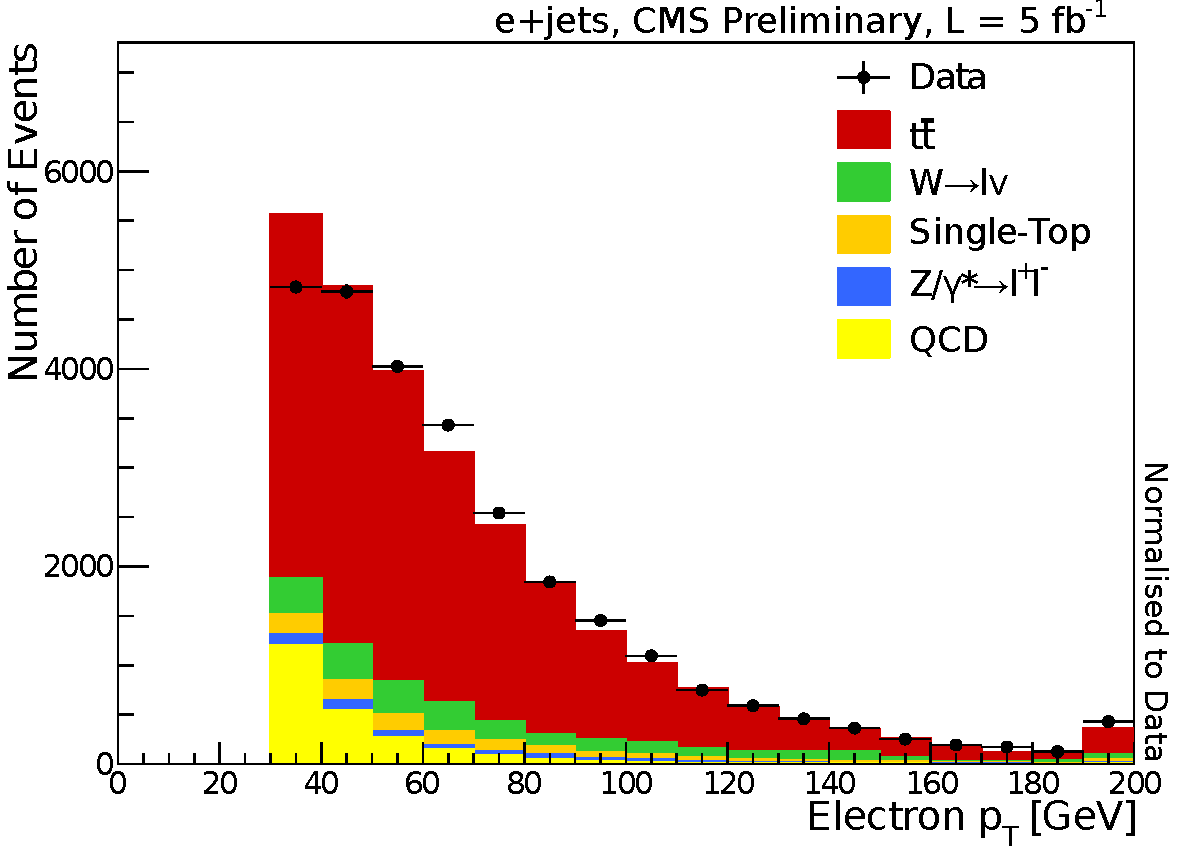
\includegraphics[width=0.5\textwidth]{cmg_electron_pt}}
   \subfloat[]{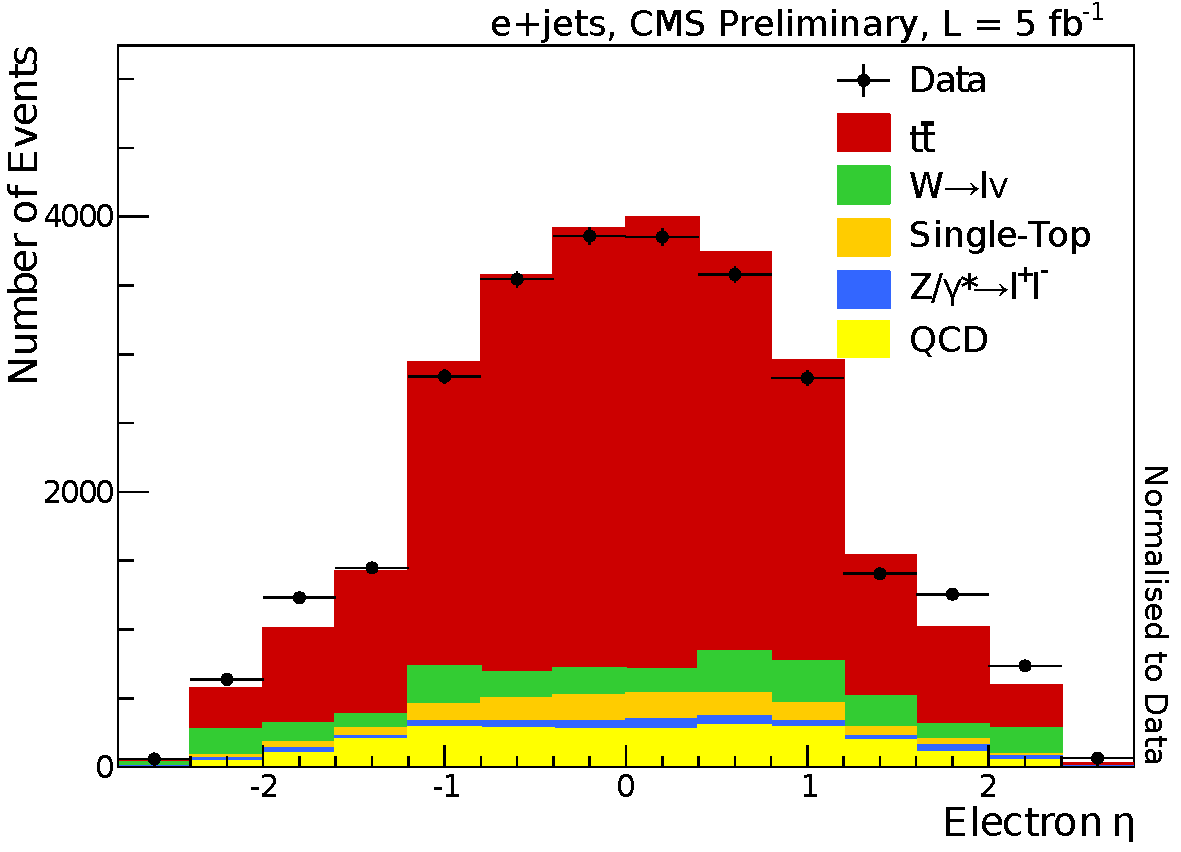
\includegraphics[width=0.5\textwidth]{cmg_electron_eta}}
   \hfill
   \subfloat[]{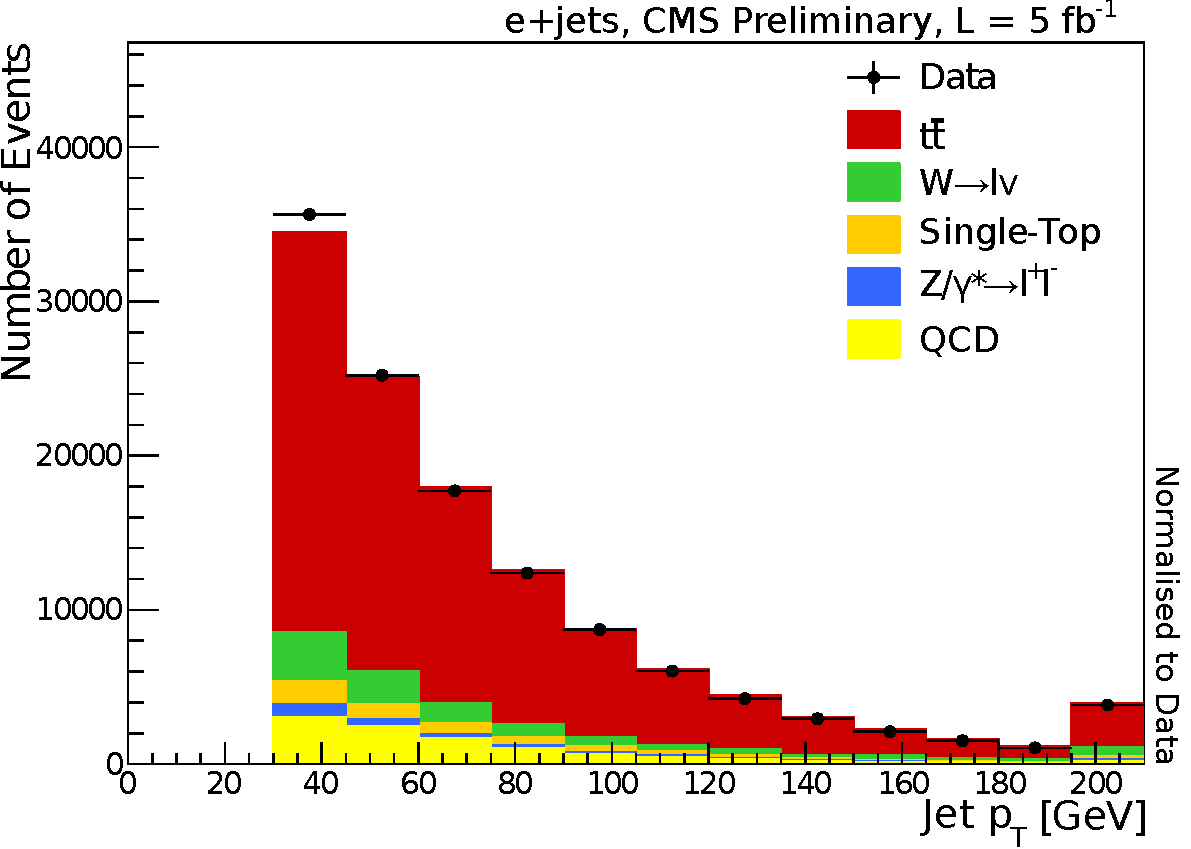
\includegraphics[width=0.5\textwidth]{cmg_jet_pt}}
   \subfloat[]{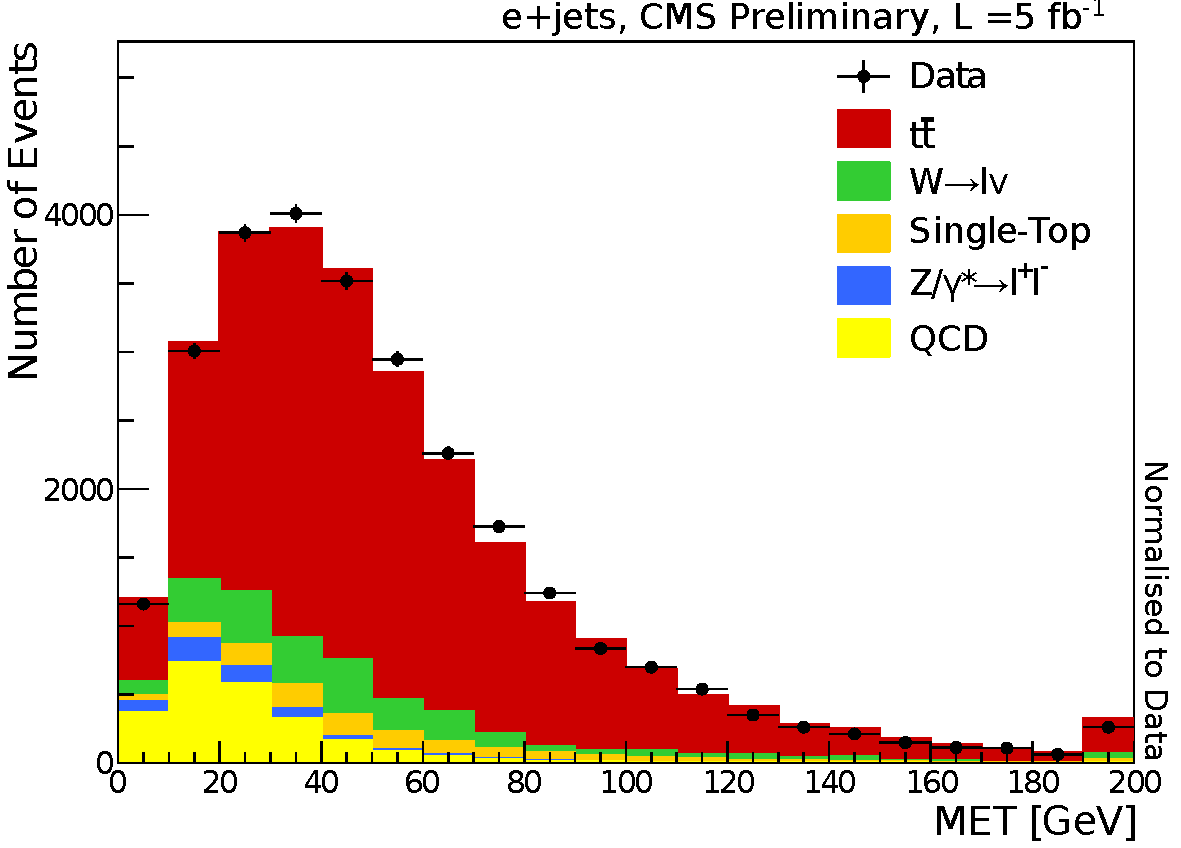
\includegraphics[width=0.5\textwidth]{cmg_met}}
   \caption{\label{fig:controlplots}Kinematic variable distributions after all selection cuts. (a) electron \pt, (b)
   electron $\eta$, (c) jet \pt for all jets passing the selection, (d) \MET.}
\end{figure}

\section{Kinematic Fit}
\label{s_top_mass:kinematic_fit}
In order to precisely measure the top quark mass, objects in the final state need to be associated with originating
partons of the top quark pair decay. In this analysis, a kinematic fit is employed to fully reconstruct the event
kinematics under the \ttbar hypothesis, thus improving the resolution of measured quantities by exploiting the knowledge
of decay process.

The \HitFit fitting package \autocite{HitFit} used in this work originates from \Dzero collaboration. Based on the SQUAW
algorithm \autocite{SQUAW} developed in Lawrence Berkeley National Laboratory, the original \HitFit code was written by
Scott Stuart Snyder in Fortran for Run I of the Tevatron. It was successfully used in the first direct measurement of
the top quark mass by \Dzero for lepton plus jets \ttbar events \autocite{D0_top_mass_1998}. The package was then
migrated to \Cplusplus for Run II of the Tevatron, and exploited in a series of \ttbar analyses including the updated
top quark mass measurement using the ideogram method \autocite{D0_top_mass_ljets_ideogram}, first measurement of the
forward-backward charge asymmetry in \ttbar production \autocite{D0_charge_assymetry} and some others.

One of the key features of the \HitFit package is its independence of specific experiments and detector geometries. The
only external dependence is on \textsc{CLHEP} \autocite{CLHEP}, a \Cplusplus library that provides utility classes for
linear algebra, geometry, vector arithmetic, etc., which was specifically developed for high energy physics simulation
and analysis software and is notably used by \GEANTfour package. In 2011 \HitFit was ported to CMSSW and later on
successfully used in a number of CMS top quark analyses, including the top mass measurement in lepton plus jets channel
\autocite{top_mass_ljets_CMS}.

\HitFit is designed to fit lepton plus jets events under the \ttbar hypothesis. Specifically, it strives to constrain
the event to a hypothesis of production of two heavy particles, each decaying into a \W boson and \cPqb quark. According
to the semi-leptonic signature, one of the \W boson decays into an electron-neutrino pair, while the other decays into a
light quark-antiquark pair.

The input to the fit includes the four-momenta of the lepton, four leading jets and missing transverse energy, as well
as their respective resolutions that were calculated using Monte Carlo samples. Since only four leading jets are used,
there are $4!=24$ ways to associate these four reconstructed jets with the partons from the \ttbar decay. The number of
permutations is reduced to $4!/2=12$ since the light jets from the hadronic \W decay are interchangeable. However, for
each hypothesis the $z$ component of neutrino four-momentum needs to be determined. This is done by requiring the two
heavy particles to have equal mass ($m_{\cPqt} = m_{\cPaqt}$), which yields to a quadratic equation which has either two
real or two complex solutions that share the real part. If case of the two real solutions the fit is performed for each
of them. If there are two complex solutions, the fit is performed once for the common real part of them, but the fit
result is included in the event content twice. Therefore, each hypothesis has two possible values of the neutrino
four-momentum, which doubles the number of permutations back to $4!=24$.

The kinematic fit is performed by minimising the $\chi^{2}$ function defined as
\begin{equation}
\chi^{2}  = (\mathbf{x} - \mathbf{x}^{m})^{T}\mathbf{G}(\mathbf{x} - \mathbf{x}^{m})
\end{equation}
where $\mathbf{x}^{m}$ is the vector or measured observables, $\mathbf{x}$ is the vector of fitted variables and
$\mathbf{G}$ is the inverse of the error matrix given by the resolutions of the observables.

The following kinematic constraints are imposed:
\begin{enumerate}[topsep=\parskip, parsep=\parskip, itemsep=\parskip, leftmargin=\leftmargin]
	\item Reconstructed top quarks from both hadronic and leptonic legs are required to have equal masses:
	\begin{equation}
		%m(t \to \ell \nu b) = m(\bar{t} \to q\bar{q} \bar{b}),
		m(\cPqt \to \ell \nu \cPqb) = m(\cPaqt \to \cPq\cPaq \cPaqb),
	\end{equation}
	\item The \W boson masses reconstructed in both hadronic and leptonic legs are fixed:
	\begin{equation}
		%m(\ell \nu) = m(q \bar{q}) = m_{W} = \SI{80.4}{\GeV}.
		m(\ell \nu) = m(\cPq\cPaq) = m_{\W} = \SI{80.4}{\GeV}.
	\end{equation}
\end{enumerate}

Apart from exploiting the knowledge of the \W mass, the \cPqb quark mass of \SI{4.7}{\GeV} is also used. Light quarks
and leptons are considered to be massless.

The full description of the fitting algorithm can be found in the appendix of the \HitFit author's PhD thesis
\autocite{Snyder}. Essentially, since the constraints are non-linear, an iterative technique is used. Starting with the
measured observables, the constraint equations are linearised by expansion in a power series around the starting point.
The minimisation is then solved with these linearised constraints, providing the new starting value for the next
minimisation step which is repeated until the $\chi^2$ converges or a maximum number of iterations is reached. Events
are rejected if there is no permutation resulting in a converging fit. Some kinematic variables for permutations giving
the best (smallest) $\chi^2$ values are shown in Figure~\ref{fig:fitplots}.

\begin{figure}[!htp]
   \centering
   \subfloat[]{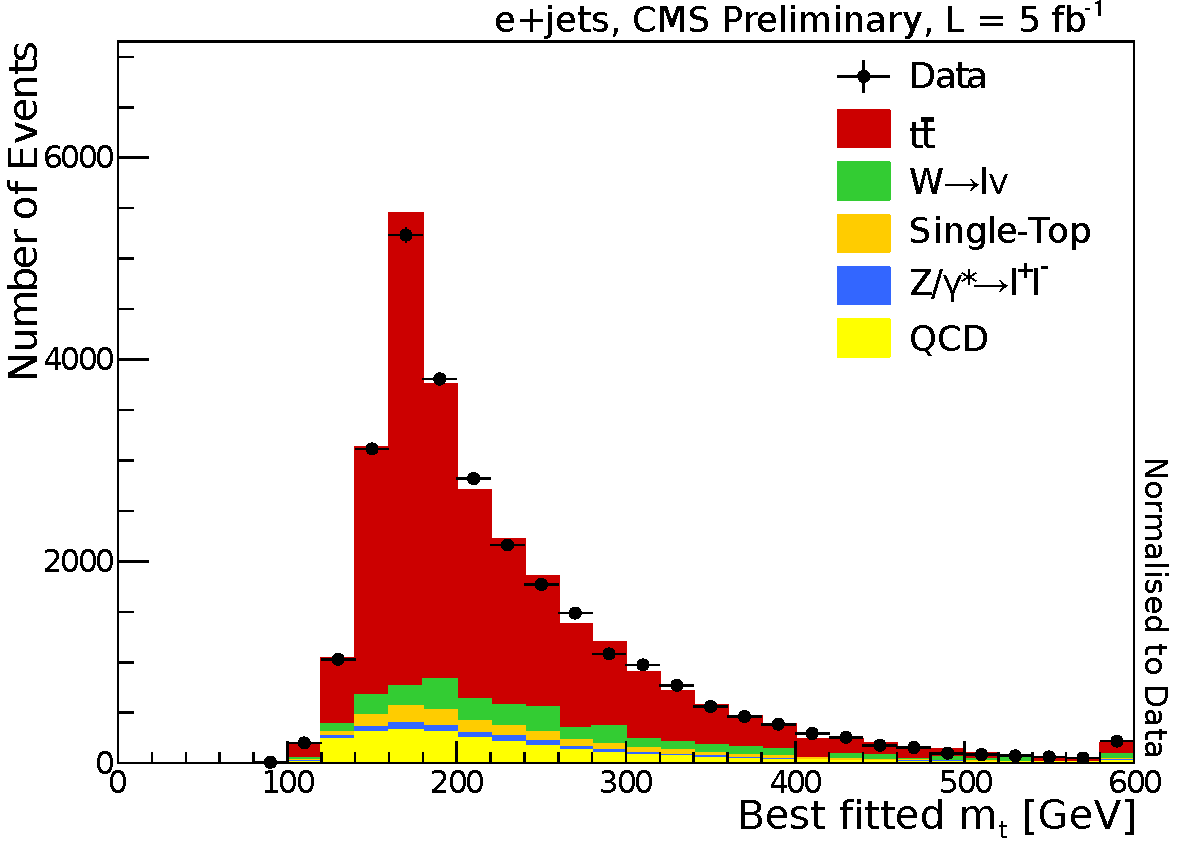
\includegraphics[width=0.5\textwidth]{hitfit_best_fitted_top_mass}}
   \subfloat[]{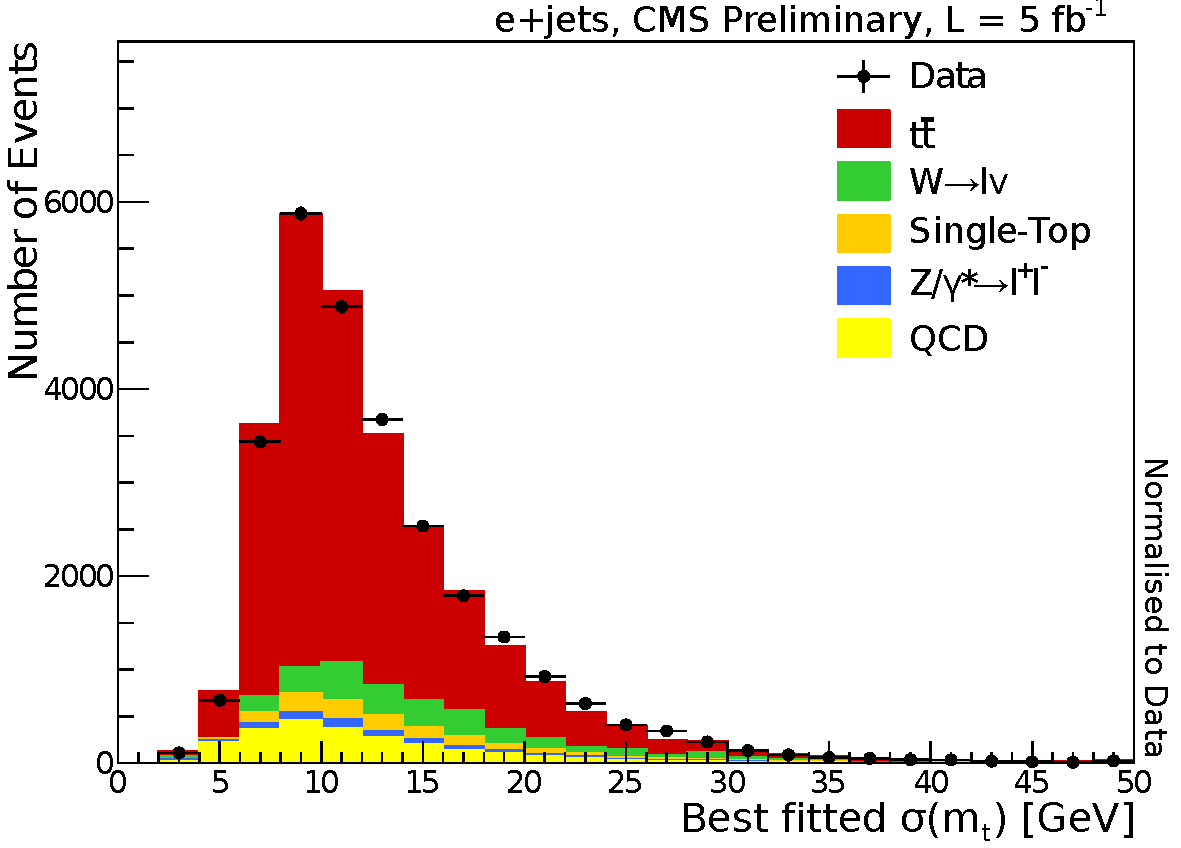
\includegraphics[width=0.5\textwidth]{hitfit_best_fitted_sigma_top_mass}}
   \hfill
   \subfloat[]{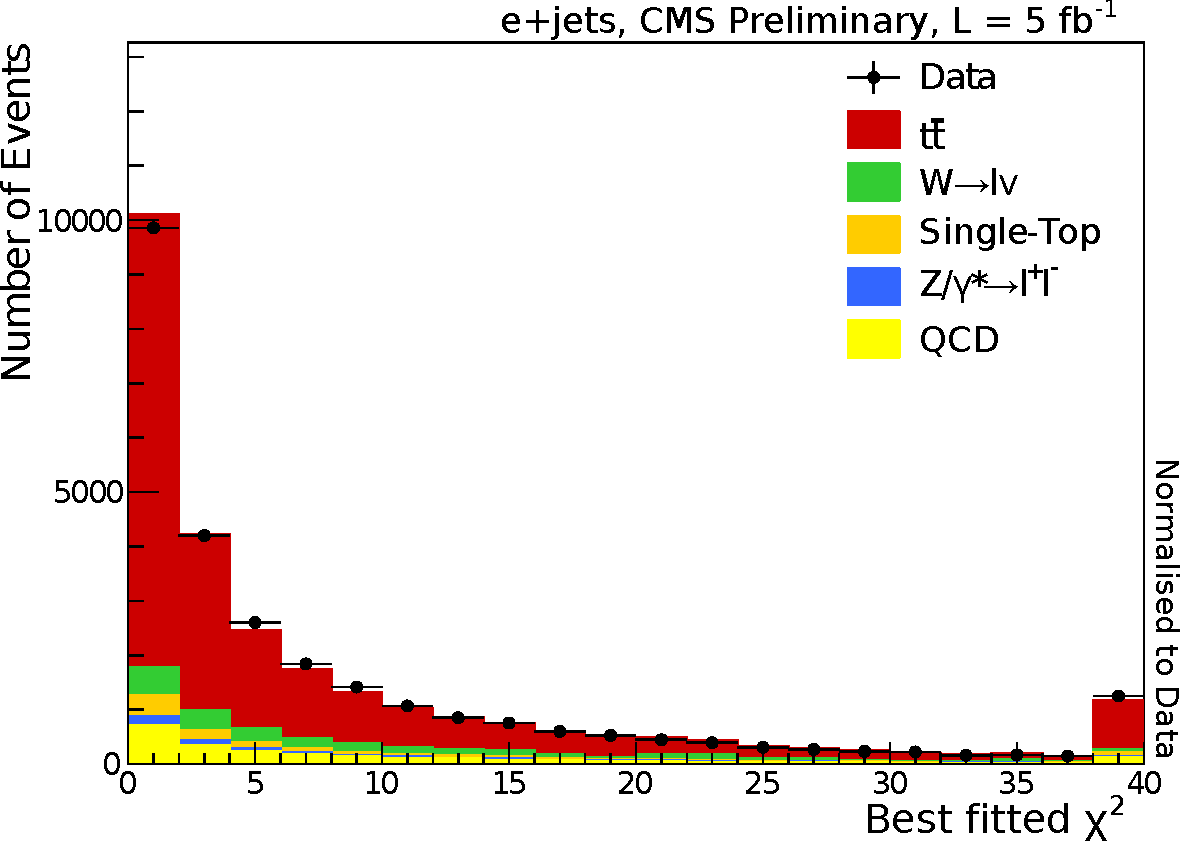
\includegraphics[width=0.5\textwidth]{hitfit_best_fitted_chi2}}
   \subfloat[]{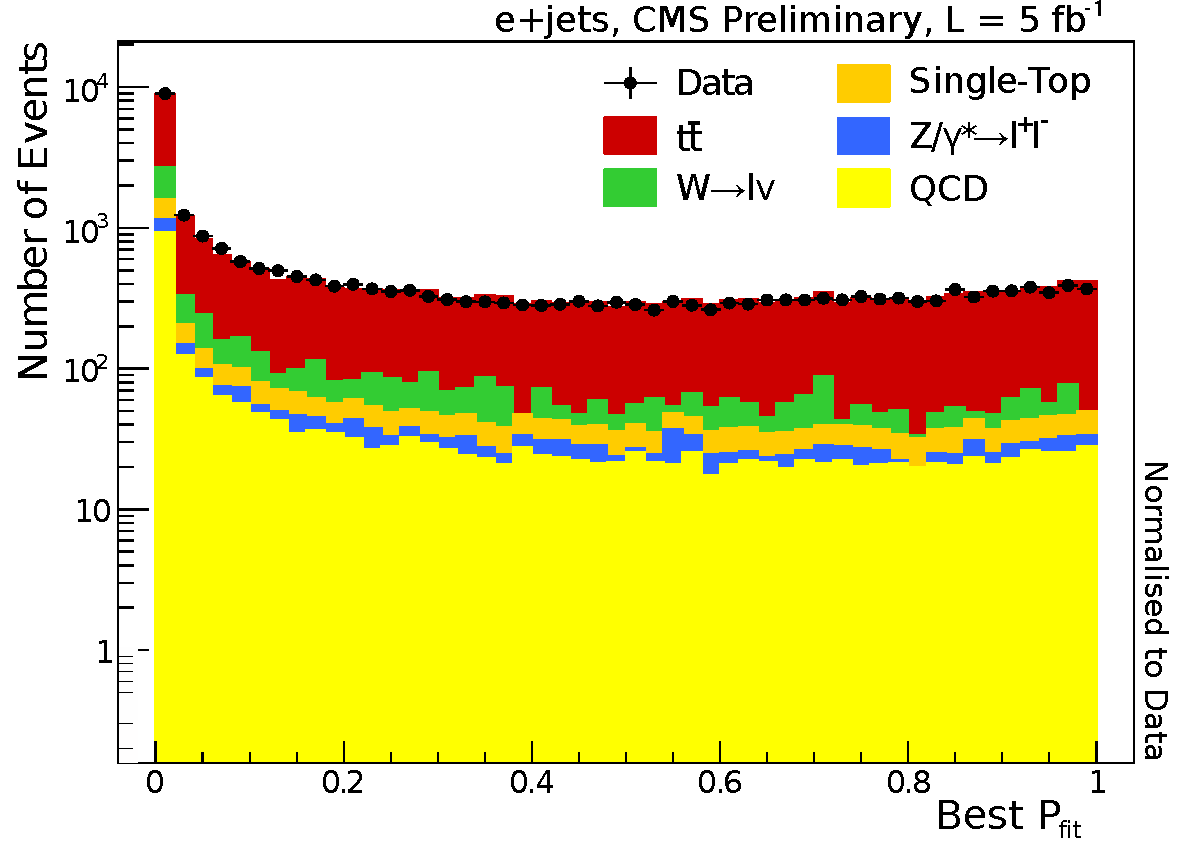
\includegraphics[width=0.5\textwidth]{hitfit_best_pfit}}
   \caption{\label{fig:fitplots}Distribution of (a) fitted top quark mass, (b) its standard deviation, (c) $\chi^{2}$
   and (d) fit probability for the best fitted hypotheses.}
\end{figure}

Typically, an event has a few permutations resulting in a converged fit. The simplest approach of picking a permutation
with the best $\chi^2$ value is disfavoured, since the Monte Carlo studies have shown that the correct permutation
does not necessarily have the best $\chi^2$. This value can change drastically with relatively small variations of the
input parameters, as different permutations may obtain the smallest value of $\chi^2$. On the other hand, some solutions
yield very large $\chi^2$ value, which typically happens for badly reconstructed or background events. Therefore, a
loose cut of $\chi^2=20$ is applied for all permutations on the output of the converged fit. This is the final
selection criteria on top of the reference selection mentioned in Section~\ref{s_top_mass:event_selection}.

%Table \ref{tab:chi2_eff} list the number of events which pass the reference selection only, and number of events which
% pass both the reference selection and the loose $\chi^{2}$ cut.

The compatibility of a permutation with the \ttbar hypothesis is quantified by the following fit probability:
\begin{equation}
	P_{\textrm{fit}} = \textrm{exp}(-\frac{1}{2}\chi^2).
\end{equation}

This probability is used in the next step of the analysis, referred to as the ideogram method.


\section{Ideogram Method}
\label{s_top_mass:ideogram_method}
The ideogram method is a powerful mass extraction technique. Its main idea lies in finding the likelihood distribution
of the particle mass given the particular data sample, which is performed by evaluating the likelihood of measured
observables given a generated particle mass for each event in the sample. The signal likelihood is evaluated from the
theoretically expected Breit-Wigner distribution convoluted with the Gaussian experimental resolution on event-by-event
basis. The whole procedure is calibrated using Monte Carlo simulation of a series of particle masses in the expected
region.

%All selected jet-parton permutations from the output of the kinematic fit are weighted by their fit probability
%$P_{\textrm{fit}}$.

One of the first applications of the ideogram method tracks back to the \W boson mass measurement by the \textsc{DELPHI}
Collaboration at CERN LEP collider \autocite{DELPHI_1998, DELPHI_2008}. It was later on used in a series of top quark
mass measurements, including the \Dzero measurement in lepton plus jets channel \autocite{D0_top_mass_ljets_ideogram}
and CDF measurement in all-hadronic channel \autocite{CDF_ideogram}. The main CMS top quark mass measurement in lepton
plus jets channel at \SI{7}{\TeV} \autocite{top_mass_ljets_CMS} which is cross-checked by this analysis is also based on
the ideogram method, however, with \textit{in situ} JES (jet energy scale) measurement in a joint likelihood fit. As JES
is a dominant systematics in this analysis, this approach proved to be more precise, but let us not neglect the
importance of a cross-check.

\subsection{Event likelihood}
\label{ss_top_mass:event_likelihood}
In the basis of the ideogram method lies the event likelihood, also referred to as the ideogram. It is calculated for
each event in the sample as a function of the hypothesised top quark mass \mtop in the following way:

\begin{equation}
\mathcal{L}_\textrm{event} \left(\mathbf{x}|\mtop, f_{\ttbar} \right) = f_{\ttbar} P_{\ttbar}
\left(\mathbf{x}|\mtop\right) + \left(1 - f_{\ttbar} \right)P_\textrm{bkg}\left(\mathbf{x}\right).
\label{eq:event_likelihood}
\end{equation}

Here $\mathbf{x}$ is the set of event observables with the top mass information from the kinematic fit, $f_{\ttbar}$ is
the fraction of \ttbar events in the data sample, and $P_{\ttbar}$ and $P_\textrm{bkg}$ are probability densities for
signal and background events, respectively. Essentially, by construction of the likelihood, the first term corresponds
to the probability for the event to be signal, whilst the second term is its probability to be background. The kinematic
information $\mathbf{x}$ includes the fitted mass $m_{i}$, the estimated standard deviation for each fitted mass
$\sigma(m_{i})$ and the goodness-of-fit $\chi^{2}_{i}$ for each permutation, i.e.\ each possible jet-parton assignment
and neutrino solution surviving the selection criteria on the output of the fit.

The \ttbar signal probability is calculated as a weighted sum over all permutations:
\begin{equation}
P_{\ttbar}\left(\mathbf{x}|\mtop\right) = \sum_{i}^{24} w_{i} \left( f_{\textrm{cp}} \cdot
\int\limits^{m_{\textrm{max}}}_{m_{\textrm{min}}} \textrm{G}\left(m'|m_{i},\sigma_{i}\right) \textrm{RBW}
\left(m'|\mtop,\Gamma_{\textrm{t}}\right) \textrm{d}m' + (1 - f_{\textrm{cp}})\textrm{WP}(m_{i}|\mtop)\right)
\end{equation}

For each permutation, the first term expresses the probability that it has a correct jet-parton assignment (correct
permutation). The second term shows the probability that it is a wrong permutation, i.e.\ the jet-parton assignment is
wrong. The relative weight $w_i$ is given as:

\begin{equation}
w_i = \textrm{exp}(-\frac{1}{2}\chi^2) w_{\rm btag}
\end{equation}

The correct-permutation probability is given as a convolution of a Gaussian resolution function
$\textrm{G}(m'|m_{i},\sigma_{i})$ and relativistic Breit-Wigner distribution
$\textrm{RBW}(m'|\mtop,\Gamma_{\textrm{t}})$. The Gaussian is centred at the value of fitted mass $m_{i}$ and has a
width of the estimated fitted mass uncertainty $\sigma_{i}$.  It describes the estimated mass resolution for each
jet/neutrino solutions. The relativistic Breit-Wigner (RBW) describes the distribution of the invariant mass $m'$ of top
quark (or antitop quark) in \ttbar event for a given assumed top quark mass $m_{t}$ and top quark width $\Gamma_{t}$.
We set the value of top quark width to 2 GeV.

We use the following form of the RBW,
\begin{equation}
RBW(m|m_{0},\Gamma_{0}) \propto \frac{m^{2}}{\left(m^{2} - m_{0}^{2}
\right)^{2} + m^{4}\frac{\Gamma_{0}^{2}}{m_{0}^{2}}}
\end{equation}
as suggested by $s-$dependence of the phase space and Standard Model electroweak corrections, see equations (1.35) and
(1.40) in \cite{:2005ema}.

% \begin{figure}[!htpb]
% \begin{center}
%     \subfigure[]{\includegraphics[width=0.49\textwidth]{figs/EJetsTtLJets1665FourJetInclCpGaussFit}}
%     \subfigure[]{\includegraphics[width=0.49\textwidth]{figs/MuJetsTtLJets1665FourJetInclCpGaussFit}}
% 	\caption{\label{fig:WJetsDensity2}
% 	Plots of the fitted mass for the \ttbar events with
%     correct-permutation.  Left is for the $e+$jets channel,
% 	right is for the $\mu$+jets channel.}
% \end{center}
% \end{figure}

The wrong-permutation probability density is derived by fitting analytical functions to the fitted mass distribution of
jet/neutrino solutions which have wrong jets to quarks assignment in Monte Carlo \ttbar event sample.  There are two
kinds of events with wrong jets to quarks assignment.  The first kind of events have the four leading jets matched to
quarks from \ttbar decay, but the jets are not assigned to quarks correctly.  The second kind of events have one or
more of the four leading jets coming from radiated gluon instead of quarks from \ttbar decay.  We found that both
type of events have similar shape and decided to group them together as events which have the wrong-permutation jets to
quarks assignment.

For each event which has at least one converging jet/neutrino solutions, we removed the jet/neutrino solutions which
have the correct jets to quarks assignment. We then plotted the fitted mass from the remaining jet/neutrino solutions.
Each entry is weighed by the same weight used in the event likelihood.

We found that the fitted mass distribution for the wrong-permutation \ttbar can be described very well by the Crystal
Ball functions with exponential order 5, with their parameters $\mu$, $\sigma$, and $\alpha$ can be parametrized as
functions of top quark mass.  Figure \ref{fig:TtWpDensity} shows the fitted mass spectra for the wrong-permutation
combinations of \ttbar events, with three different masses: 166.5, 172.5, and 178.5 GeV.

% \begin{figure}[!htpb]
% \begin{center}
%     \subfigure[]{\includegraphics[width=0.41\textwidth]{figs/CbFitTagWpm4jiEJetsTtLJets1665}}
%     \subfigure[]{\includegraphics[width=0.41\textwidth]{figs/CbFitTagWpm4jiMuJetsTtLJets1665}}

%     \subfigure[]{\includegraphics[width=0.41\textwidth]{figs/CbFitTagWpm4jiEJetsTtLJets1725}}
%     \subfigure[]{\includegraphics[width=0.41\textwidth]{figs/CbFitTagWpm4jiMuJetsTtLJets1725}}

%     \subfigure[]{\includegraphics[width=0.41\textwidth]{figs/CbFitTagWpm4jiEJetsTtLJets1785}}
%     \subfigure[]{\includegraphics[width=0.41\textwidth]{figs/CbFitTagWpm4jiMuJetsTtLJets1785}}
% 	\caption{\label{fig:TtWpDensity}
% 	Plots of the fitted mass for the \ttbar events with
%     wrong-permutation. Left is
% 	for the $e+$jets channel, right is for the $\mu$+jets channel.  Top
%     row is for $m_{t} = 166.5$ GeV, middle row is for $m_{t} = 172.5$
%     GeV, bottom row is for $m_{t} = 178.5$ GeV.}
% \end{center}
% \end{figure}

\subsection{Background probability}

The shapes of the background probability are taken from the fitted mass spectrum in $W+$jets Monte Carlo samples. We
perform the kinematic fit to $W+$jets Monte Carlo events and plot all fitted mass for all jet permutations, weighted by
the $\chi^{2}$ and b-tagging weights as described before.  We found that the fitted mass spectra of $W+$jets events can
be described by a Landau distribution, with different parametrization for $e$+jets and $\mu$+jets channel.  Figure
\ref{fig:WJetsDensity} shows the fitted mass spectra for the $W+$jets events.


The background probability density only depends on $x$ and doesn't depend on $m_{t}$.  We assume that the background
probability can be described by the probability density for $W+$jets events only. The contributions from $W+$ heavy
flavour jets, single top, $Z+$jets, and QCD events are expected to be small.  Furthermore, their probability densities
have similar shape to that of $W+$jets events. Note that in the final MC calibration we include all above backgrounds to
evaluate and correct for a possible bias due to this (and other) approximation(s).

The probabilities are calculated as a weighted sum over all possible combinations of jet to quark assignments and
neutrino solutions.  The relative probability for each solution to fulfil the \ttbar lepton+jets event hypothesis
is proportional to $\exp\left(-\frac{1}{2}\chi^{2}\right)$.  However, some solutions yield very large $\chi^{2}$ value
from the kinematic fit. Those are mostly either badly misreconstructed events or background events which don't carry top
quark mass information.  Therefore, we take only solutions which have $\chi^{2}$ value from the kinematic fit smaller
than 20.

% \begin{figure}[!htpb]
% \begin{center}
%     \subfigure[]{\includegraphics[width=0.49\textwidth]{figs/EJetsWJetsFourJetInclMass}}
%     \subfigure[]{\includegraphics[width=0.49\textwidth]{figs/MuJetsWJetsFourJetInclMass}}
% 	\caption{\label{fig:WJetsDensity}
% 	Plots of the fitted mass in $W+$jets sample.  Left is
% 	for the $e+$jets channel, right is for the $\mu$+jets channel.}
% \end{center}
% \end{figure}

\subsection{Inclusion of b-tagging information in the likelihood}

This analysis uses b-tagging information to further separate
\ttbar signal and background, and to separate \ttbar signal with correct and wrong jet permutation assignments.  We use
the Combined Secondary Vertex (CSV) tagging algorithm at the Medium working point (requiring CSV discriminant to be
greater than 0.679).
%This %is the same algorithm and working point used by the reference \ttbar %cross-section with b-tagging analysis
%\cite{CMS-PAS-TOP-11-003???}.

If one or more jets in the event is b-tagged, we assign an additional relative weight, $w_{\rm btag}$, representing the
likelihood that the observed b-tags are compatible with the jet flavour assignment hypothesis for that particular jet
permutation.

\begin{equation}
w_{\rm btag} = \prod_{j} p^{j}
\end{equation}

where the index $j$ runs over all the jets considered in the fit.  The b tag probability $p^{j}$ can be either
$\varepsilon_{l}$, $(1 - \varepsilon_{l})$, $\varepsilon_{b}$, or $(1 - \varepsilon_{b})$, depending on the hypothesized
flavour of the jet (light jet or b jet), and whether the jet is b-tagged or not.  For the light jet mistag rate, we
assume that the $W boson$ can decay into $c\bar{s}$ and $u\bar{d}$ pair, and thus take into account the higher tagging
rate for c quark jet.


\subsection{Combined likelihood fit}
\label{ss_top_mass:likelihood_fit}

The likelihood for the entire lepton+jets sample is calculated as the product of each event likelihood curve,
\begin{equation}
\mathcal{L}_{sample} = \prod_{\rm all~event}
\mathcal{L}_{event}\left(x|m_{t},f_{t\bar{t}}\right).
\label{eq:CombinedLikelihood}
\end{equation}
Difference in sample composition between subsamples ($e$+jets and $\mu$+jets, 0-tag and 1-tag and 2-tag) are taken into
account in the likelihood.

In practice, what is done is summing over the negative likelihood for all events in the sample.  For each event, the
likelihood is evaluated as a function of top quark mass.  The minima of the sum of log likelihood curve is then taken as
the most probable value of top quark mass.

\section{Mass calibration}
\label{s_top_mass:calibration}

\section{Systematic Uncertainties}
\label{s_top_mass:systematics}

\section{Results}
\label{s_top_mass:results}

\section{Summary}
\label{s_top_mass:summary}


% ------------------------------------------------------------------------


%%% Local Variables: 
%%% mode: latex
%%% TeX-master: "../thesis"
%%% End: 
